\documentclass[slidestop,compress,mathserif]{beamer}
\usepackage[latin1]{inputenc}
\usepackage{verbatim}
\usepackage{graphicx}
\usetheme{Boadilla}
\usecolortheme{beaver} %{beetle}%{crane} 
\usepackage{textpos}
\usepackage{tikz}
\usepackage{biblatex}
\bibliography{foo}


\title[Compact Muon Solenoid]{General Info: Luminosity}
\author[Ramkrishna Sharma]{{\bf Ramkrishna Sharma},Md. Naimuddin}
\institute[DU]{University of Delhi, India}
\date{\today}

\setbeamertemplate{footline}[slide number]
\setbeamertemplate{frametitle}[default][center]         % For centering the Heading

\titlegraphic{
	
\includegraphics[width=1.5cm,keepaspectratio]{cern.jpg}\hspace*{3.35cm}~%
	
\includegraphics[width=2cm,keepaspectratio]{logo_du.jpeg}\hspace*{2.75cm}~%
	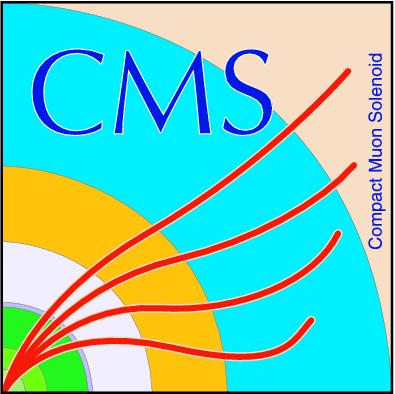
\includegraphics[width=1.5cm,keepaspectratio]{cmsLogo.jpeg}
}

\begin{document}
\renewcommand{\inserttotalframenumber}{\pageref{lastslide}}
\begin{frame}
\titlepage
\end{frame}

\begin{frame}\frametitle{Table of contents}\tableofcontents
\end{frame}
%%%%%%%%%%%%%%%%%%%%%%%%%%%%%%%%%%%%%%%%%%%%%%%%%%%%%%%%%%%%%%%%%%%%%%%%%%%%%%%%%%%%%%%%%%%%%%%%%%%%%%%
\section{Introduction}


\begin{comment}

\begin{frame}\frametitle{}

\end{frame}

\begin{frame}\frametitle{}
	\begin{center}
	\includegraphics[width=6.5cm]{}
	\end{center}
\end{frame}

\subsection{LHC Layout}
\begin{frame}\frametitle{LHC Layouts}\fontsize{9pt}{7.5}\selectfont
	\begin{columns}[T]
	\column{.5\textwidth}
		\begin{block}{}
			\begin{center}

			\end{center}
		\end{block}

	\column{.45\textwidth}   
		\begin{block}{}
		\begin{itemize}
		  \item
		\end{itemize}
		\end{block}
	\end{columns}
\end{frame}

\end{comment}


\label{lastslide}
\begin{frame}[c]
	\begin{center}
	\Huge Thanks
	\end{center}
\end{frame}

\begin{frame}[c]
	\begin{center}
	\Huge Backup Slides
	\end{center}
\end{frame}



\end{document}
